\documentclass[a4paper, oneside]{article}

\usepackage[T1]{fontenc}
\usepackage[utf8]{inputenc}
\usepackage[italian]{babel}
\usepackage{frontespizio}
\usepackage{graphicx}
\usepackage{listings}
\usepackage{scrextend}
\usepackage[margin=1.2in]{geometry}
\usepackage[font=small,labelfont=bf]{caption}

\begin{document}

\baselineskip 13pt
	
% ---- FRONTESPIZIO ----- 
\begin{frontespizio} 
 \Preambolo{\renewcommand{\frontpretitlefont}{\fontsize{15}{12}\scshape}}
\Istituzione {University of Pisa}
\Divisione {Scuola di Ingegneria}
\Corso [Laurea]{Artificial Intelligence and Data Engineering}
\Annoaccademico {2019--2020}
\Titolo { \vspace {35mm}Task0 documentation}
\Filigrana [height=4cm,before=0.28,after=1]{./images/stemma_unipi.png}
\Rientro {1cm}
\Candidato {Alice Nannini}
\Candidato {Giacomo Mantovani}
\Candidato {Marco Parola}
\Candidato {Stefano Poleggi}
\Relatore {Prof. Pietro Ducange}
 \Punteggiatura {}
\end{frontespizio}

\clearpage

% ----- INDICE -----
	\tableofcontents
	\clearpage


\section{Introduction}
This is an application to browse and evaluate university courses and professors, called \textbf{Student-Evaluation}.\\
The application is developed to allow students (users) to view all the courses and professors of a specific university with related comments.\\ 
There are two buttons to switch the view of the list of professors to the list of courses: this action will update the table below. By clicking an element of this table, on the left section, the user can see more information about the chosen element: general information and comments.\\ 
In order to filter the list of professors and subjects, there is a choice box, thanks to which the user can select a specific degree course. \\
In order to leave a comment, it is necessary to log in, otherwise, the application will allow interaction in read-only.\\
There are two buttons in the bottom left corner to allow students to update or delete their comments.
There is no form to register into the application, it is assumed that users are already registered into the system, but there is an administrator that can add, update and delete professors, subjects and  all the informations related.


\begin{minipage}{\linewidth}
\begin{center}
\vspace{8mm}
\includegraphics[width=150mm]{./images/diagrams/Mockup.pdf} 
\vspace{3mm}
\captionof{figure}{Mockup}
\label{fig:mockup}
\end{center}
\end{minipage}

\clearpage

% ----- REQUIREMENTS -----
\section{Requirements}


\subsection{Functional requirement}
The system has to allow the guest to carry out basic functions such as:
\begin{itemize}
\item To select a course/professor from the list and view information and comments.
\item To select a degree course from the list, filtering professors and subjects.
\end{itemize}
In addiction to the guest functions, the system has to allow the user to carry out basic functions such as:
\begin{itemize}
\item To login into the system.
\item To upload comments on a course/professor.
\item To update a comment of a course/professor only if the user is the owner.
\item To delete a comment of a course/professor only if the user is the owner.
\end{itemize}
\vspace{2mm}
The system has to allow the administrator to carry out basic functions such as:
\begin{itemize}
\item To login into the system.
\item To add a course/professor.
\item To update a course/professor.
\item To delete a course/professor.
\item To associate to a course a professor.
\item To delete any comment.
\end{itemize}
\vspace{2mm}

\subsection{Non-functional requirements}
\begin{itemize}
\item Usability, ease of use and intuitiveness of the application by the user.
\item Avaliable, the service is guarantee h24.
\item The system shall support up to 2000 simultaneous users.
\item The system should provide access to the database with no more than 10 seconds of latency.
\end{itemize}

\clearpage

% ----- USE CASES -----
\section{Use case}

\textbf{Actors}
\begin{itemize}
\item{Guest : this actor represents a user who is not logged into the system}
\item{Student : this actor represents a user who is logged into the system}
\item{Admin : this actor represents the administrator of the system}
\end{itemize}

\subsection{Use Cases Description}
The actions of this application are:\\
\textbf{Log In}: This use case describes how the user logs into the StudentEvaluation system.\\
\textbf{Log out}: This use case describes how the user exits from StudentEvaluation system.\\
\textbf{Browse professors}: This use case describes how the system retrieve all the professors\\
\textbf{Find professor}: This use case describes the selection of a single professor from the list\\
\textbf{View professor}: This use case allows a user to view the informations about a professor.\\
\textbf{Browse subjects}: This use case describes how the system retrieve all the subjects\\
\textbf{Find subject}: This use case describes the selection of a single subject from the list\\
\textbf{View subject}: This use case allows a user to view the informations about a subject.\\
\textbf{Browse degree courses}: This use case describes how the system retrieve all the degree courses\\
\textbf{Find degree course}: This use case describes the selection of a single degree course from the list\\
\textbf{Add prof/subject}: This use case allows an admin to add a professor/subject to related list.\\
\textbf{Update prof/subject}: This use case allows an admin to modify the informations related to a professor/subject.\\
\textbf{Delete prof/subject}: This use case allows an admin to remove a professor/subject from related list.\\
\textbf{Add comment}: This use case allows a user to add a comment on a professor/subject.\\
\textbf{Browse comments}: This use case describes how the system retrieve all the comments\\
\textbf{Find comment}: This use case describes the selection of a single comment from the list\\
\textbf{View comment}: This use case allows a user to view the informations about a comment.\\
\textbf{Delete Comment}: This use case allows a user to delete his comment from a professor/course list.\\
\textbf{Update Comment}: This use case allows a user to update his comment relatet to a professor/course.\\


\begin{minipage}{\linewidth}
\begin{center}
\vspace{8mm}
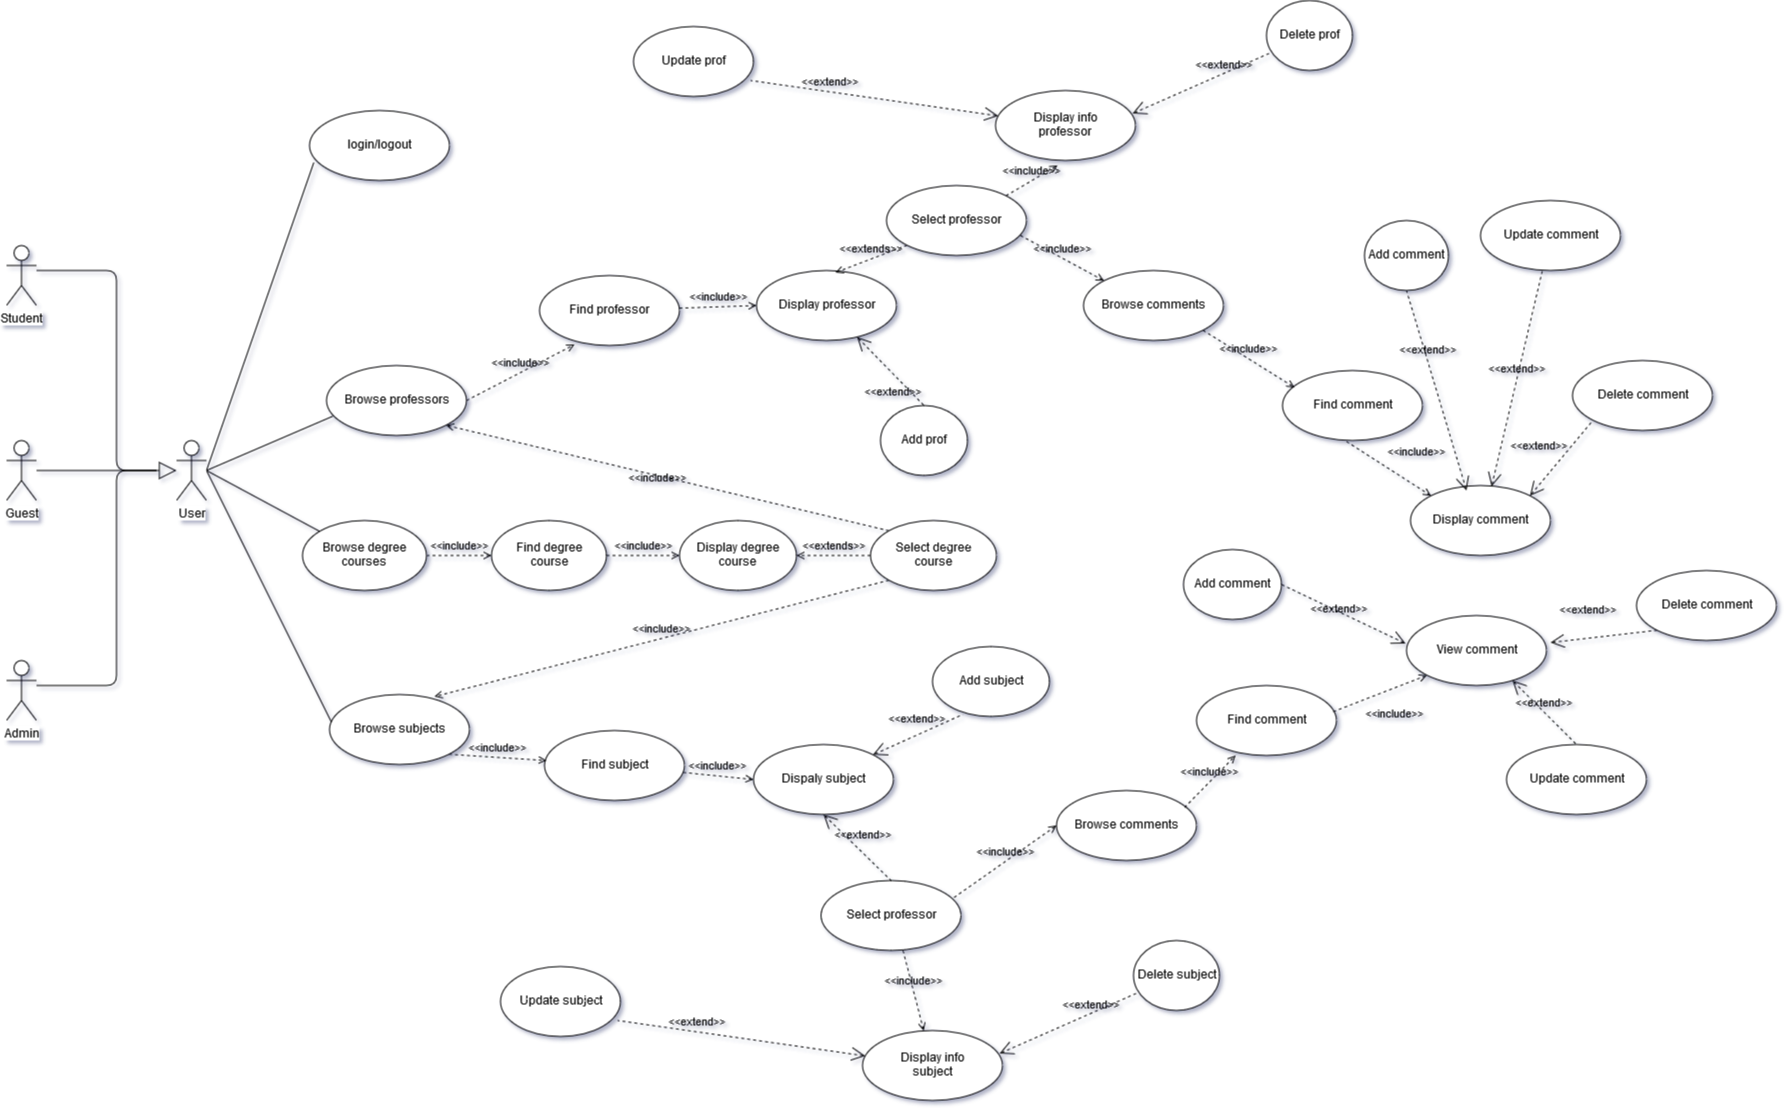
\includegraphics[ height=150mm, angle=90]{./images/diagrams/UseCases.png} 
\vspace{3mm}
\end{center}
\end{minipage}


\clearpage


\section{Calss diagram}
This diagram represent the main entities of the application and the relations between them.
\begin{minipage}{\linewidth}
\begin{center}
\vspace{4mm}
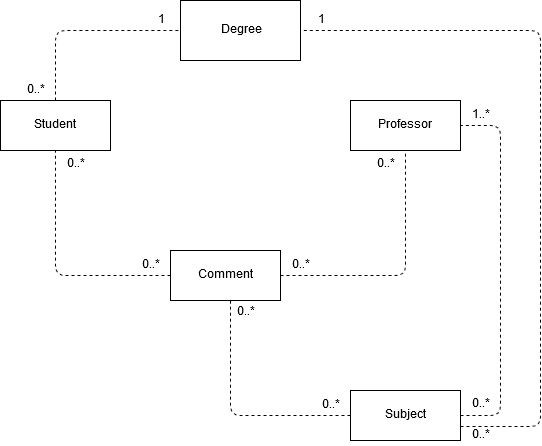
\includegraphics[width = 0.7\textwidth]{./images/diagrams/AnalysisUML.png} 
\vspace{2mm}
\captionof{figure}{UML analysis diagram}
\label{fig:useCases}
\end{center}
\end{minipage}
\clearpage
% ----- DESIGN -----
\section{Design}

\subsection{Software architecture}
The application is designed over 3 different layers, see figure \ref{fig:architecture_diagram}:
\begin{itemize}
\item Front-end
\item Middleware
\item Back-end
\end{itemize}
\vspace{5mm}
\begin{minipage}{\linewidth}
\begin{center}
\vspace{1mm}
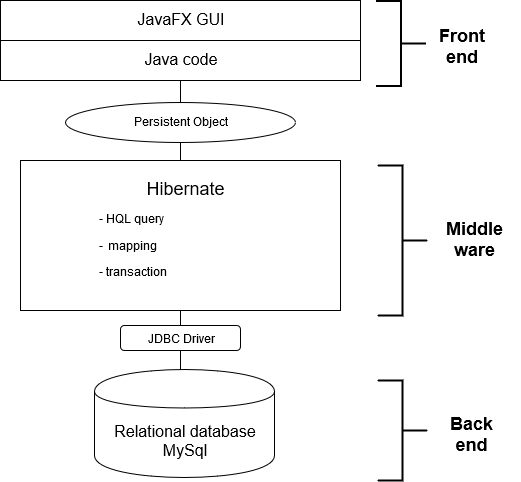
\includegraphics[height = 100mm]{./images/diagrams/architecture_diagram.png} 
\vspace{6mm}
\captionof{figure}{Software architecture diagram\\}
\label{fig:architecture_diagram}
\end{center}
\end{minipage}
\vspace{5mm}

\clearpage
\subsection{Database design}
The application is developped over a relational-database, using the MySql platform. The figure \ref{fig:diagramma_er} shows the ER-diagram of the database.\\

\begin{minipage}{\linewidth}
\begin{center}
\vspace{1mm}
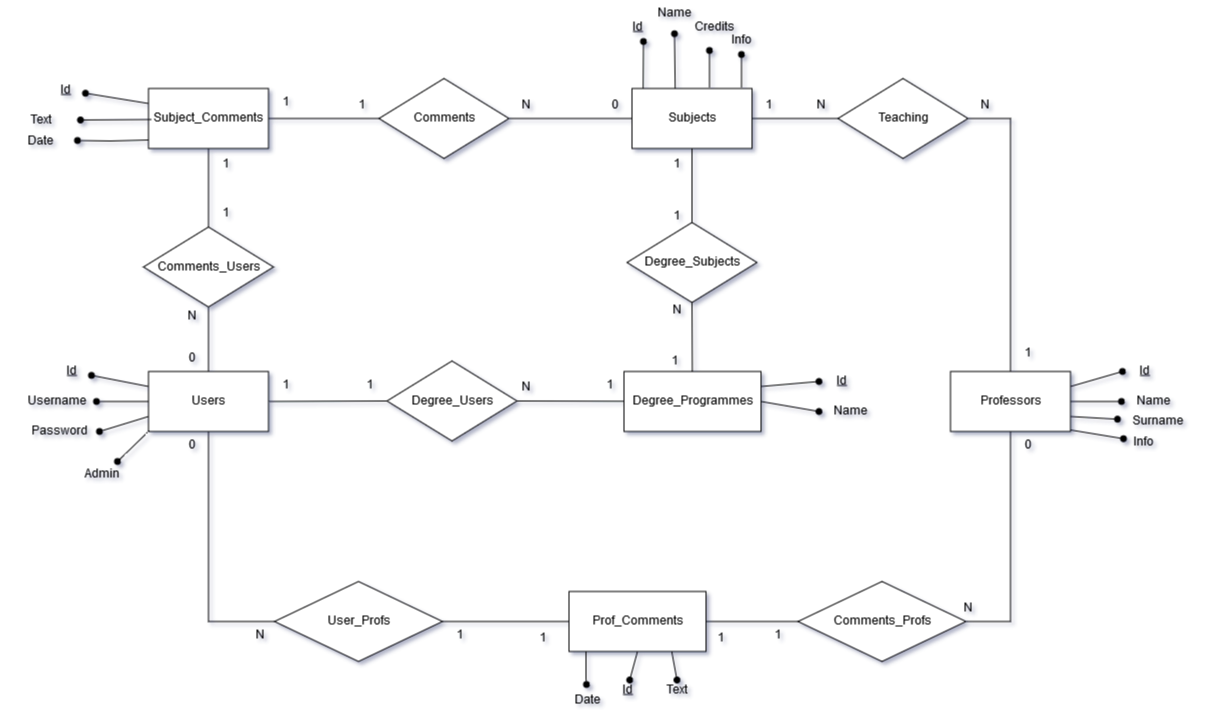
\includegraphics[width=155mm]{./images/diagrams/er_diagram.png} 
\vspace{2mm}
\captionof{figure}{ER diagram\\}
\label{fig:diagramma_er}
\end{center}
\end{minipage}

\vspace{19mm}



\clearpage
% ----- IMPLEMENTATION -----


\section{Implementation}
\subsection{Used technologies}
The application is developed in java programming language, version 11.0.4, and in JavaFX system to create the GUI, version 11, so it should run on each platform in which JVM is installed, but the application is tested and guardantee on Ubuntu 16 and Window OS. Moreover Maven is used  to build and mantain the project, version 3.8.0. \\
The middleware layer is built thanks to Hibernate, version 5.4.4.0.\\
The jdbc driver manage the comunication between middleware layer and backend layer, version 8.0.17.\\ 
For the backend layer it is used Apache as web-server, version 2.4 (including Php, MySql).\\
So this application is tested using these technologies, considering these particular versions: for other versions the correct execution isn't guaranteed .
\subsection{Snippets of code}
This phase describes the most interesting parts about the creation and interaction with the database.\\
The following classes are mapped in the table of the database: 

\begin{itemize}	
\item Degree
\item Student
\item Professor
\item Subject
\item ProfessorComment
\item ProfessotSubject
\end{itemize}
These classes are declared using the Hibernate annotations syntax.\\
The following java-code shows a declaration of the class Subject as example, and contains the annotations used also in the other classes.

\vspace{2mm}
% ----- android wearable module -----
\begin{lstlisting}[language=Java,  basicstyle=\footnotesize]
@Entity(name = "Subjects")
@Table(name = "subjects")
public class Subject {

	@Column(name = "id")
	@Id
	@GeneratedValue(strategy = GenerationType.IDENTITY)
	private int id;
	private String name;
	private int credits;
	@Column(name = "info", columnDefinition="TEXT")
	private String info;

	// relation with degree
	@ManyToOne(fetch = FetchType.LAZY)
	@JoinColumn(name = "degreeId")
	private Degree deg;

	// relation with Subject comments.
	@OneToMany(mappedBy = "subj", cascade = CascadeType.ALL, orphanRemoval = true)
	private List<SubjectComment> subjectComments = new ArrayList<SubjectComment>();

	// relation with Professors.
	@ManyToMany
	@JoinTable(name = "teaching", joinColumns = @JoinColumn(name = "subjectId"),
		 inverseJoinColumns = @JoinColumn(name = "profId"))
	private Set<Professor> professor = new HashSet<Professor>();
\end{lstlisting}
\vspace{5mm}

\begin{minipage}{\linewidth}
\begin{center}
\vspace{1mm}
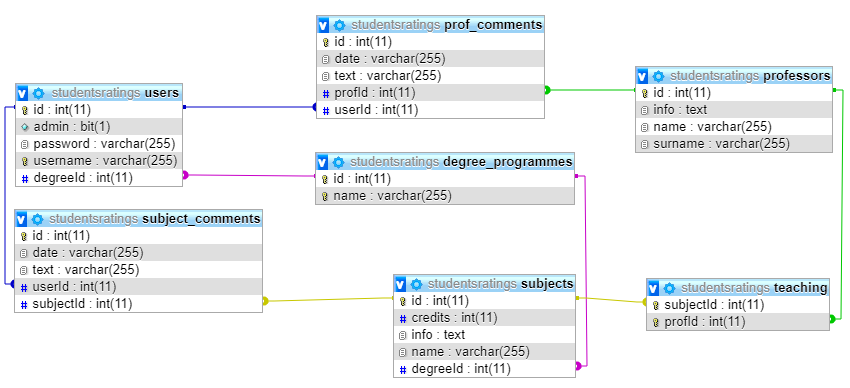
\includegraphics[width=155mm]{./images/diagrams/er_diagram2.png} 
\captionof{figure}{ER diagram\\}
\label{fig:diagramma_er2}
\end{center}
\end{minipage}
\vspace{5mm}\\
 Another foundamental class is ManagerEM, that manages the db-connection and the related operations.
 The implementation of a set of CRUD operations, regarding the class Subject, is desribed as follows.

\subsection{Create}
Creating a new subject specifying general informations, the professor holding the course and the associated degree program as parameters.\\
\vspace{2mm}
% ----- android wearable module -----
\begin{lstlisting}[language=Java,  basicstyle=\footnotesize]
public Subject createSubject(String name, int credits, String info, 
					String profIdStr, int degreeId){
	System.out.println("Creating a new subject");

	Subject subject = new Subject(0, name, credits, info);
	String[] professorsId = profIdStr.split(",", 5);
	try {
		entityManager = factory.createEntityManager();
		Degree degree = entityManager.find(Degree.class, degreeId);
		int profId = 0;
		for (String p : professorsId) {
			profId = Integer.parseInt(p);
			Professor professor = null;
			if (profId > 0) {
				professor = entityManager.find(Professor.class, profId);
			}
			if (profId > 0 && professor == null) {
				System.err.println("the inserted prof Id doesn't exixst");
				entityManager.close();
				return null;
			}
			subject.getProfessor().add(professor);
			professor.getSubject().add(subject);
		}
		degree.getSubject().add(subject);
		subject.setDeg(degree);

		entityManager.getTransaction().begin();
		entityManager.persist(subject);
		entityManager.getTransaction().commit();
		System.out.println("subject Added");
		return subject;

	} catch (Exception ex) {
		ex.printStackTrace();
		System.err.println("A problem occurred in updating a subject!");
	} finally {
		entityManager.close();
	}
	return subject;

}
\end{lstlisting}
\vspace{5mm}

\subsection{Read}
This functionality returns a list of subjects interrogating the database using a query written in Hibernate Query Language (HQL).\\
\vspace{2mm}
% ----- android wearable module -----
\begin{lstlisting}[language=Java,  basicstyle=\footnotesize]
public List<Subject> getSubjects(int degree) {

	List<Subject> results = new ArrayList<>();
	String selectionSubjectByDegree = "SELECT s" +
					"FROM Subjects s" + 
					"WHERE degreeId = ?1" +
					"ORDER BY s.name";
	try {
	   entityManager = factory.createEntityManager();
           TypedQuery<Subject> query = entityManager.createQuery(selectionSubjectByDegree,
							 	 Subject.class);
           query.setParameter(1, degree);
           results = query.getResultList();
	} 
        ...
        return results;
}
\end{lstlisting}
\vspace{5mm}

\subsection{Update}
This operation allows students to update their comments about a selected subject.\\
\vspace{2mm}
% ----- android wearable module -----
\begin{lstlisting}[language=Java,  basicstyle=\footnotesize]
public boolean updateCommentSubject(int subjectCommentId, String text, int userId) {
	System.out.println("Updating a subject comment");
	boolean updated = false;
	Date date = new Date();

	try {
		entityManager = factory.createEntityManager();
		SubjectComment subjectComment = entityManager.find
					(SubjectComment.class, subjectCommentId);

		// if the user is the owner.
		if (subjectComment.getStud().getId() == userId) {
			entityManager.getTransaction().begin();
			subjectComment.setText(text);
			subjectComment.setDate(date);
			entityManager.getTransaction().commit();
			System.out.println("subject comment updated");
			updated = true;

		} else { // if user is not owner --> error
			System.err.println("You are not the owner of that comment,
					 please select another comment");
			entityManager.close();
			return updated;
		}
	} catch (Exception ex) {
		ex.printStackTrace();
		System.err.println("A problem occurred in updating a subject comment!");

	} finally {
		entityManager.close();
	}
	return updated;
}
\end{lstlisting}
\vspace{5mm}

\subsection{Delete}
This operation allows a student to delete their comments about a selected subject.\\
\vspace{2mm}
% ----- android wearable module -----
\begin{lstlisting}[language=Java,  basicstyle=\footnotesize]
public boolean deleteCommentSubject(int subjectCommentId, int userId, boolean admin) {
	boolean deleted = false;
	try {
		entityManager = factory.createEntityManager();
		entityManager.getTransaction().begin();
		SubjectComment subjectComment = entityManager.find(SubjectComment.class,
								   subjectCommentId);

		if (subjectComment.getStud().getId() == userId) {
			entityManager.remove(subjectComment);
                entityManager.getTransaction().commit();
			deleted = true;
		} else {
                entityManager.close();
			return deleted;
		}
	} 
        ...
	return deleted;
}
\end{lstlisting}
\vspace{5mm}

\subsection{GUI}
Moreover there are 3 classes to manage the graphic user interface: 
\begin{itemize}
\item GraphicInterface
\item CommentTable
\item ProfSubjectTable
\end{itemize}
 These classes use the javaFX framework to build the GUI and handle the related events.

\clearpage


% ----- LEVEL DB -----
\section{Level DB}

An alternative implementation of this application developed using MySql relational database, can be done using a key-value database, so in this chapter is describe an implementation of the application using levelDB.\\
Key-values databases are one of the simplest examples of NoSQL stores that can be found. In a key-value database, data are persistently stored assigning a value to a uniqle identifier, which takes the name of key; couples of key-values are stored in namespaces (buckets) and in each buckets, keys must be unique. The main strenghts of the key-value database are:
\begin{itemize}
\item Simplicity
\item Speed 
\item Scalability
\end{itemize}
Key-value database are mostly used when speed in retrieving data and ease of storage are more important than the organization of data into complex structures. So, in general, classics RDBMS are preferred when organization and management is more important than perfomances; typically, when a database presents a lot of relations among entities, key-values stores aren’t the best choice. When the structure of our database is simple, instead, we could use the key-value stores because they are more capable of providing higher performances than RDBMS.\\
It is also true that simple relations between entities are represented in key-value database as well, just by building up keys in a predefined way.\\
The application we realized is a multi-users one, so it needs a remote and shared database, to whom every users can access at every moment. LevelDB does not support remote usage (differently from other key-value database), so it is not feasible to re-implement our kind of application realizing that tool. Moreover, one of the strenght of LevelDB is the possibility to handle flexibile data, but in our case the data does not vary a lot from their original structure (etc. NULL value are not expected etc.). In conclusion we don’t have many advantages in replicate the application in a key-value architecture.\\
For illustrative purpose, we tried to recreate the structure of our application using LevelDB.
First of all, we needed to define the key structure for our entities; to do so, we have choosen to represent the tables in our buckets using the table name, the id of the object we are referring to and the attribute name for the value.
Let’s consider our “users” table, used to store information about the users of our application.\\

\begin{minipage}{\linewidth}
\begin{center}
\vspace{4mm}
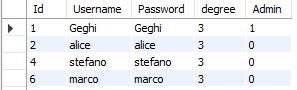
\includegraphics[width = 0.6\textwidth]{./images/table/users.jpg} 
\vspace{2mm}
\captionof{figure}{Users table}
\label{fig:tableUsers}
\end{center}
\vspace{3mm}
\end{minipage}
In key-value database we use keys to retrieve value of our objects. To define the three main components of the key (prefix, identifiers and suffix), we extract those information from the entity. So, we use the entity name (users) to define the prefix, the id (called user\_id) as the identifiers of the key and the suffix is specified by its related attribute. Our schema can be represented by a group of key-value pair specified as follows:\\
\begin{center}
	\textbf{user:\$user\_id:\$attribute\_name = \$value}
\end{center}
\vspace{5mm}
The table “users” becomes:
\vspace{2mm} \\
Users:1:Username = “Geghi”\\
Users:1:Password =  “Geghi”\\
Users:1:degree = “3”\\
Users:1:Admin = “1”\\
Users:2:Username = “alice”\\
Users:2:Password = “alice”\\
Users:2:degree = “3”\\
Users:2:Admin = “0”\\
Users:4:Username = “stefano”\\
Users:4:Password = “stefano”\\
Users:4:degree = “3”\\
Users:4:Admin = “0”\\
Users:6:Username = “marco”\\
Users:6:Password = “marco”\\
Users:6:degree = “3”\\
Users:6:Admin = “0”\\
\vspace{3mm} \\
Relations among entities are respresented in RDBMS with foreign keys. We used a similar approach in translating relational database into key-value schema. The foreign key becomes an addictional identifier in the key for the pair.\\
For that example, we focus on the tale “subject\_comments” that contains the comment of the user about subject. Among the others, we store in that table informations regard the user that made the comment (using his id) and the subject of the comment (using the id of that subject).\\
\begin{minipage}{\linewidth}
\begin{center}
\vspace{4mm}
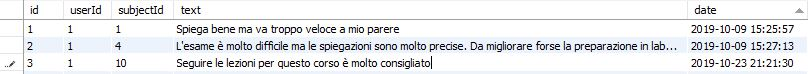
\includegraphics[width = 1\textwidth]{./images/table/subject_comments.jpg} 
\vspace{2mm}
\captionof{figure}{Subject comments table}
\label{fig:subjectCommTable}
\end{center}
\vspace{3mm}
\end{minipage}
We can see the userId, foreign key related to the user who made the comment, and subjectID, foreign key of the subject.\\
To represent that relation, the identifiers of the key becomes the id of the comment (subject\_comment\_id) the user id (user\_id) and the subject id (subject\_id).\\ The prefix is again the name of the entity and the suffix is the name of the fields. The table is represented by a group of key-value pair specified as follow:
\begin{center}
\textbf{subject\_comments:\$subject\_comment\_id:\$user\_id:\$subject\_id:\$attribute\_name = \$value}
\end{center}
\vspace{5mm}
The table “subject\_comments” become:
\vspace{2mm} \\
Subject\_comments:1:1:1:text = “Spiega bene ma va troppo veloce a mio parere”\\
Subject\_comments:1:1:1:date = “2019-10-09 15:25:57”\\
Subject\_comments:2:1:4:text = “L’esame è molto difficile ma le spiegazioni sono  … “\\
Subject\_comments:2:1:4:date = “2019-10-09 15:27:13”\\
Subject\_comments:3:1:10:text = “Seguire le lezioni per questo corso è molto consigliato”\\
Subject\_comments:3:1:10:date = “2019-10-23 21:21:30”\\
\vspace{2mm} \\
LevelDB saves the key-value pairs in a file, to initializate that file it is necessary to istantiate the class DB, Option and File, that will provide the tool to works with this architecture. That task must be computed only the first time, so we put the “init.txt” file into the folder project. At every start, the application will check that file, but only the first time we run the code it will istantiate all the buckets; after that initialization, it will update the file writing “true” on it.\\
Here is the snippet of the code used in our application to create, initializate and populate the buckets with some basic informations.
\vspace{3mm}
% ----- android wearable module -----
\begin{lstlisting}[language=Java,  basicstyle=\footnotesize]
  DB levelDBStore;
  Options options = new Options();
  File f = new File("levelDBStore");
  levelDBStore = factory.open(f, options);
    	
    	//key -> users:$user_id:$attribute_name
  levelDBStore.put("users:1:username".getBytes(), "Geghi".getBytes());
  levelDBStore.put("users:1:password".getBytes(), "Geghi".getBytes());
  levelDBStore.put("users:1:degree".getBytes(), "3".getBytes());
  levelDBStore.put("users:1:admin".getBytes(), "1".getBytes());

\end{lstlisting}
\vspace{5mm}
In order to convert the “teaching” table, representing an N-M relation in RDBMS, to a key-value schema, we introduced a new atribute, changing a bit the structure of the table. Thanks to that table we can map the relation among subjects and professors who teach them.\\
\begin{minipage}{\linewidth}
\begin{center}
\vspace{4mm}
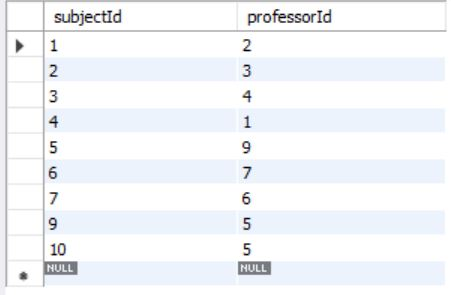
\includegraphics[width = 0.4\textwidth]{./images/table/teaching.jpg} 
\vspace{2mm}
\captionof{figure}{Teaching table}
\label{fig:teachingTable}
\end{center}
\vspace{3mm}
\end{minipage}
The key for that table becomes:
\begin{center}
\textbf{teaching:\$subjectId:professorId = \$value}
\end{center}
where \$value represents the role of the professor in the teaching of that subject.



\clearpage
% ----- MANUAL -----
\section{User Manual}
When you first run the application, the interface you get is the one in figure~\ref{fig:screen0}. 

\begin{figure}[h]
\centering
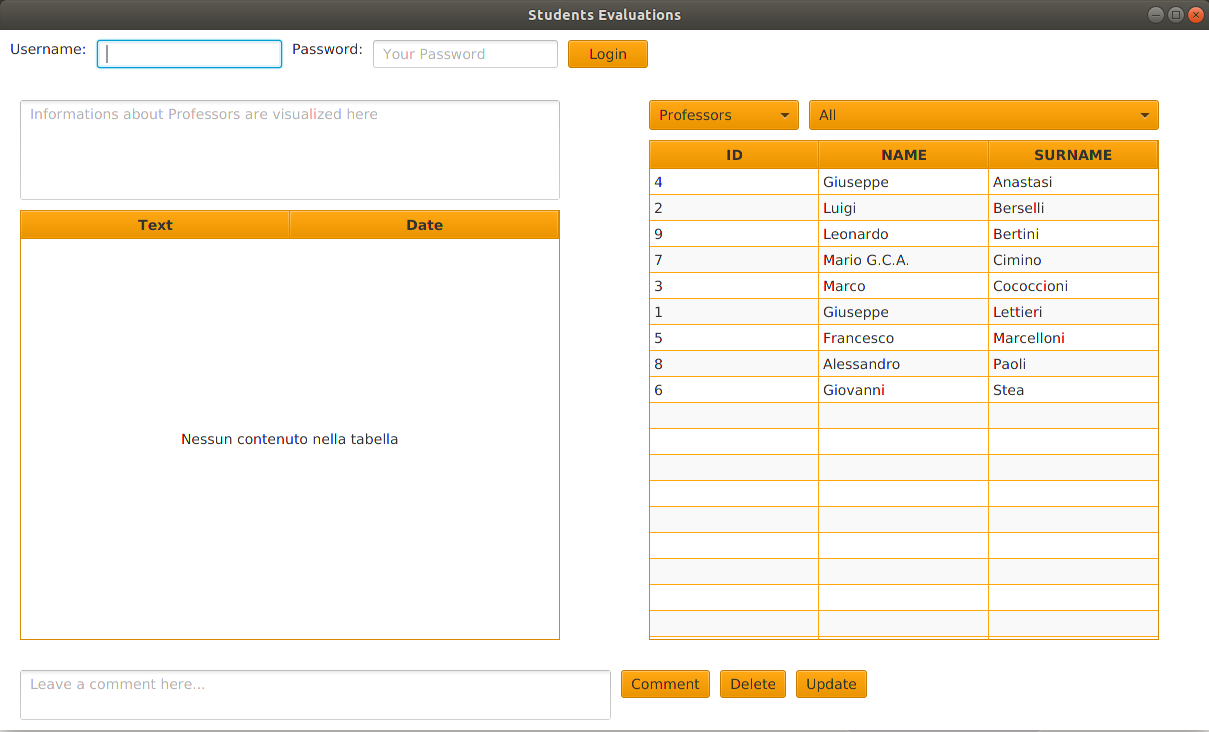
\includegraphics[width=0.88\textwidth]{images/screens/screen0}
\captionof{figure}{First view of the application}
\label{fig:screen0}
\end{figure}

The default display includes the list of all registered professors in the table on the right. You can choose to display the professors of a single degree course, using the drop-down menu on the right (fig.~\ref{fig:screen1}), or decide to view the list of subjects (fig.~\ref{fig:screen2}), for which is also available the degree course's filter. 

\begin{figure}[h]
\centering
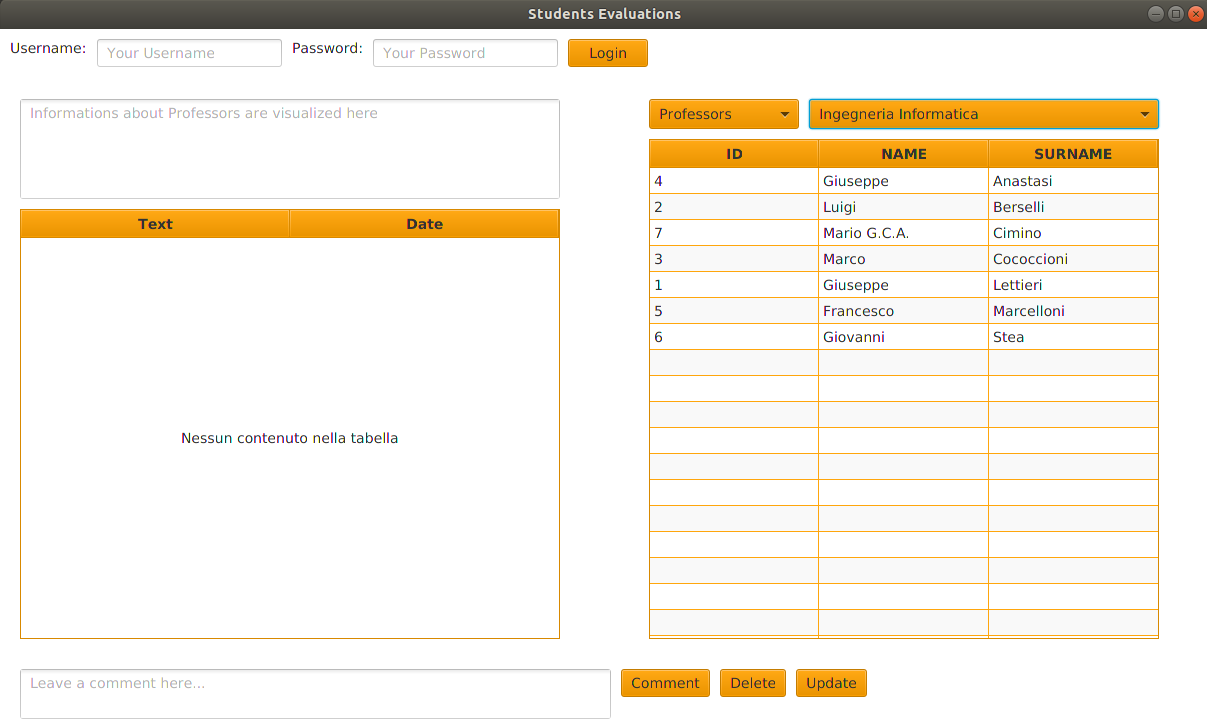
\includegraphics[width=0.88\textwidth]{images/screens/screen1}
\captionof{figure}{Selection of professors filtered by "Ingegneria Informatica" degree course}
\label{fig:screen1}
\end{figure}
\clearpage
\begin{figure}[h]
\centering
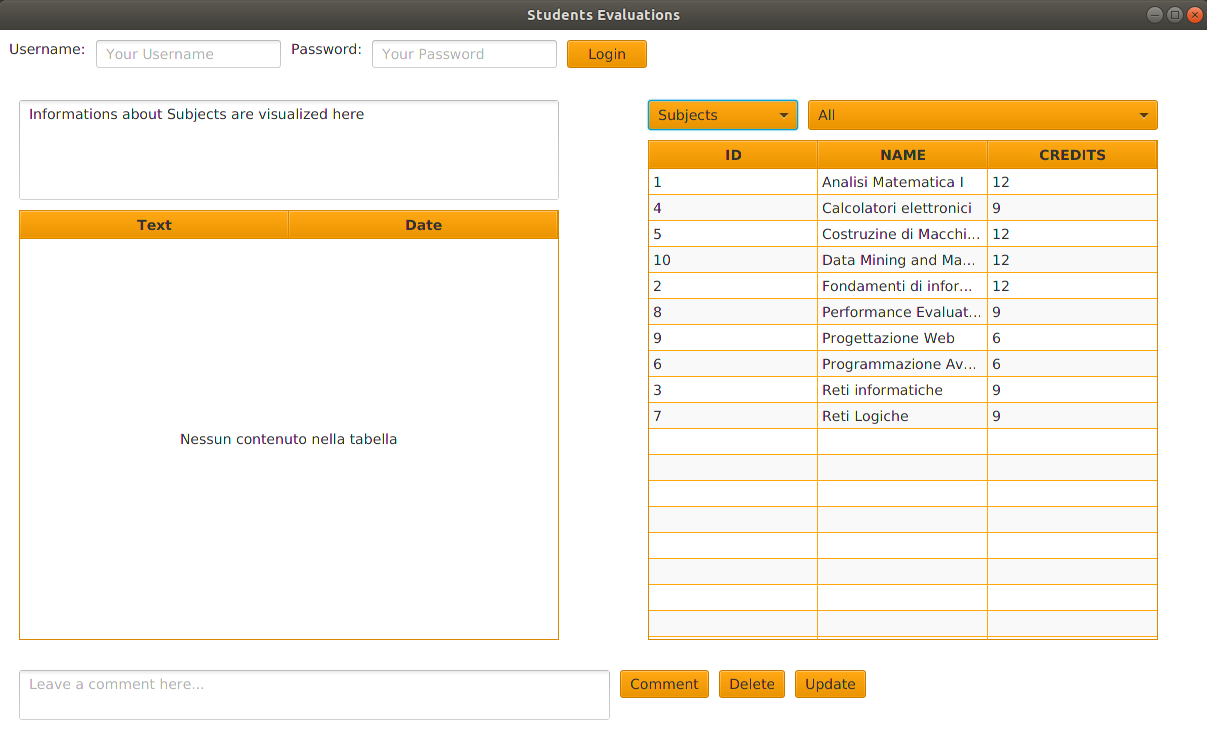
\includegraphics[width=0.88\textwidth]{images/screens/screen2}
\captionof{figure}{Selection of subjects}
\label{fig:screen2}
\end{figure}

If you have a registered account, you can log in to the application, so that the comments' operations aren't blocked. Enter your username and your password in the suited fields at the top and click on "Login" (fig.~\ref{fig:screenLogin}).
\begin{figure}[h]
\centering
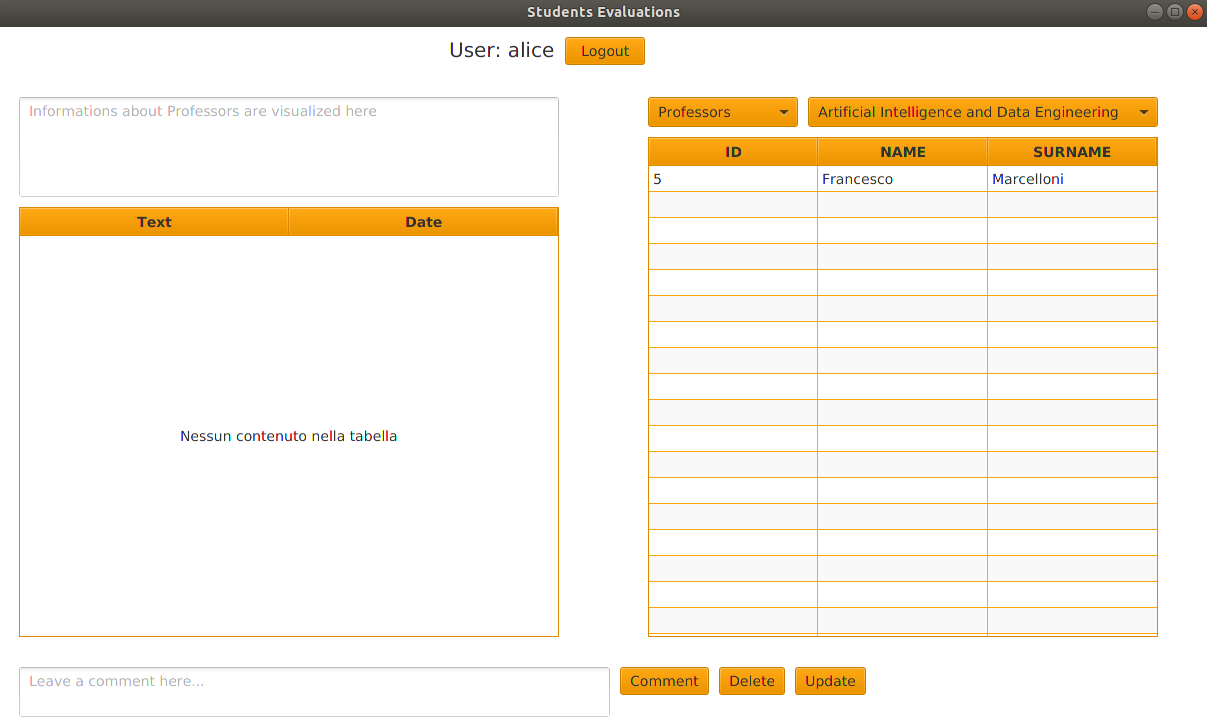
\includegraphics[width=0.88\textwidth]{images/screens/screenLogin}
\captionof{figure}{Application interface after the user "Alice" has logged in}
\label{fig:screenLogin}
\end{figure}

If you now want to be able to see the comments associated with a particular professor, you have to click on the name of the professor: in the table on the left the list of comments already received will appear (fig.~\ref{fig:screen3}). With this operation, you'll be able to visualize also the information related to that professor.

To leave a comment, you need to enter the text in the field below the table and then click on the "Comment" button. The result obtained from these operations is shown in fig.~\ref{fig:screen4}.

\begin{figure}
\centering
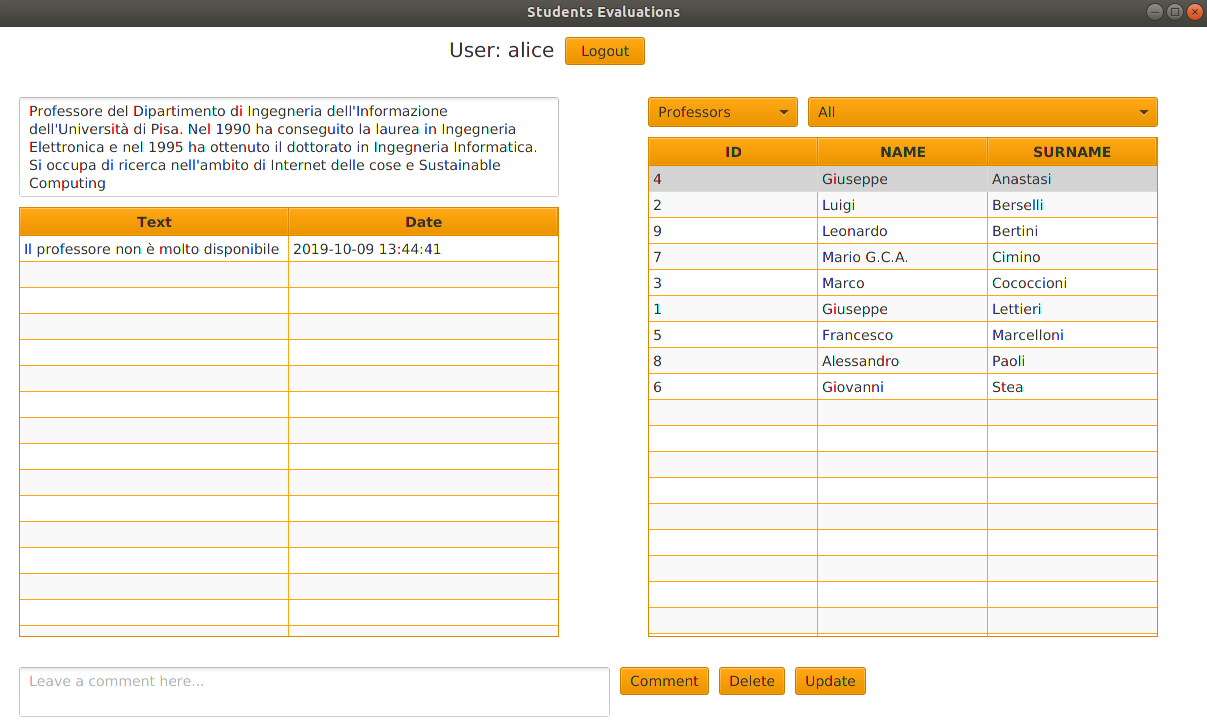
\includegraphics[width=0.9\textwidth]{images/screens/screen3}
\captionof{figure}{Displaying the comments related to a professor}
\label{fig:screen3}
\end{figure}

\begin{figure}
\centering
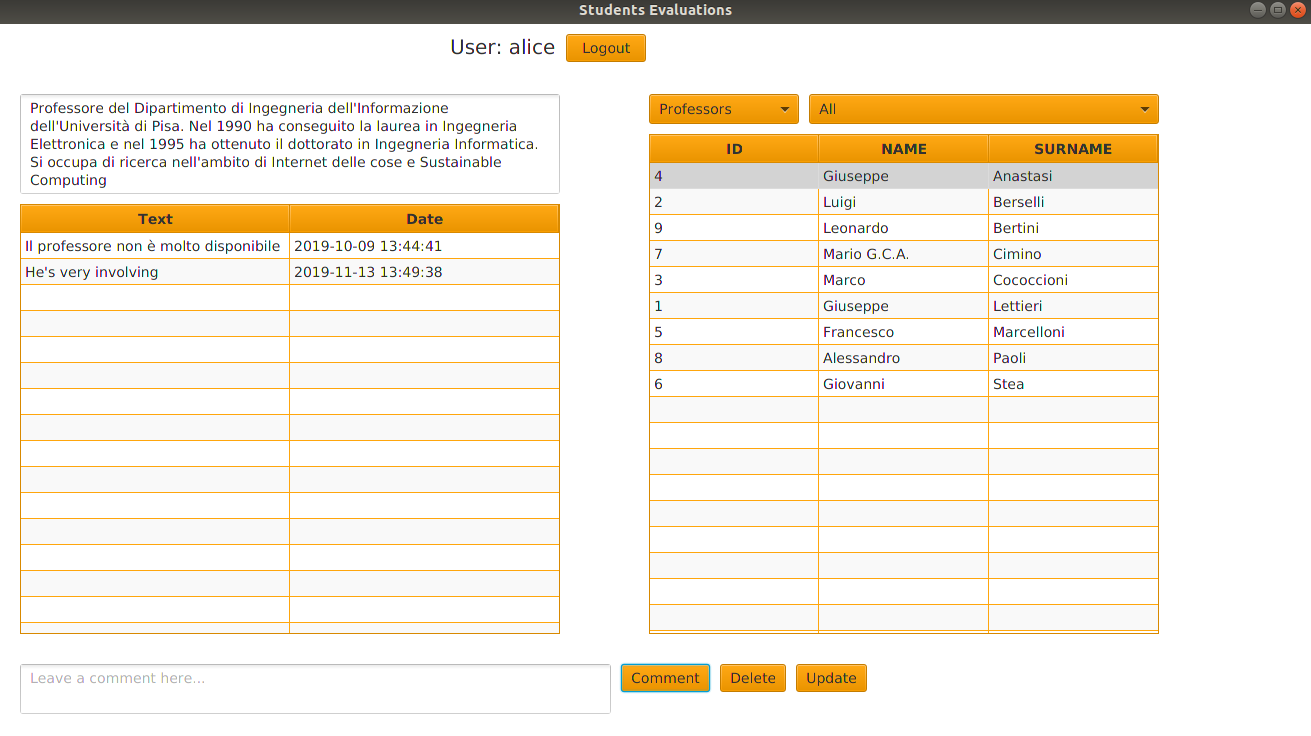
\includegraphics[width=0.9\textwidth]{images/screens/screen4}
\captionof{figure}{Interface after adding a comment}
\label{fig:screen4}
\end{figure}

You can also decide to modify the comment you just uploaded or another comment you made on a previous session. To do so, you need to click on the comment you want to update, change the text in the field below the table and then click on the "Update" button (fig.~\ref{fig:screen5}).
Finally you have the chance to delete your comment, by clicking on "Delete" after selecting it. Notice that you can modify or delete just the comments that you made.

The operations of adding, updating and deleting work as well for the the subjects' comments.
\begin{figure}[h]
\centering
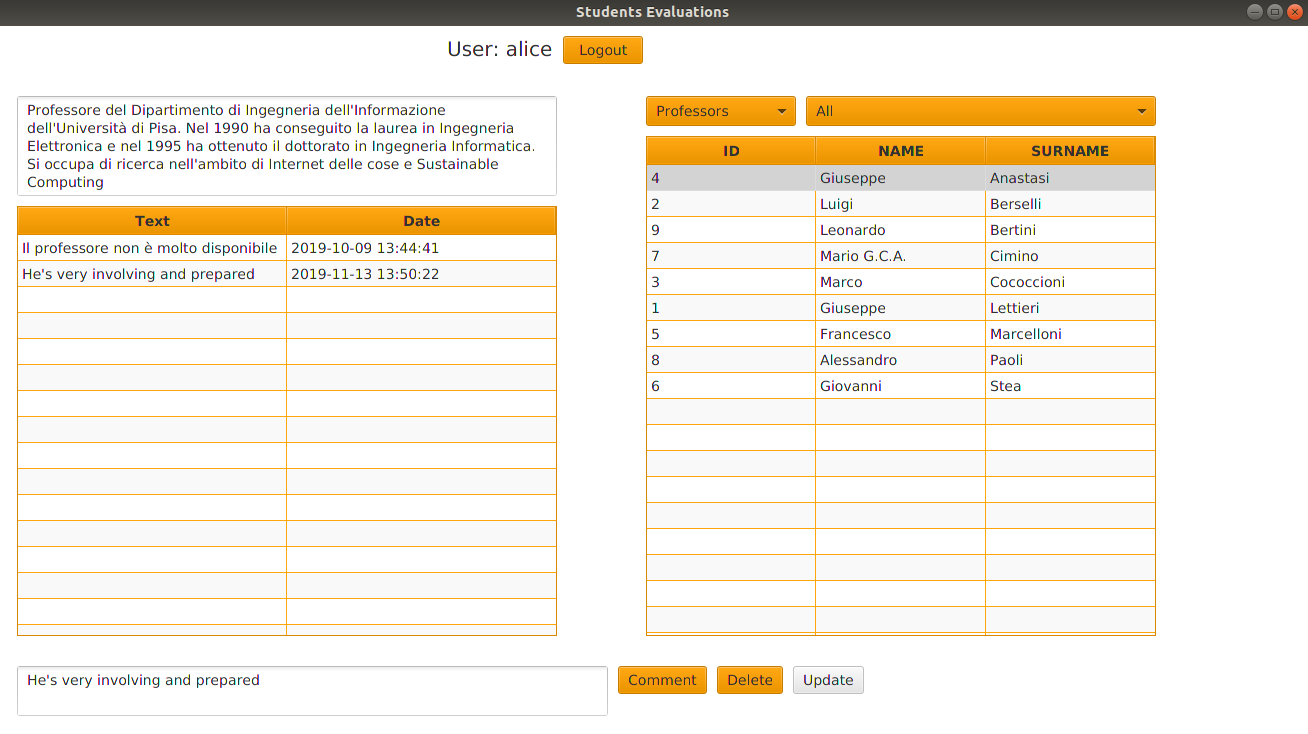
\includegraphics[width=0.88\textwidth]{images/screens/screen5}
\captionof{figure}{Interface after updating a comment}
\label{fig:screen5}
\end{figure}

To log out, just click on the appropriate button at the top, next to the user label.

Moreover, if you don't have a registered username, you can still browse through the application, search for professors 'and subjects' information and read all comments. You are just unable to leave or change any comments.

\clearpage
%ADIMN MANUAL%
\subsection{Admin Manual}
If you have an admin user, you are entitled to make changes both on the professors' and the subjects' lists. You need to log in inserting your username and password, and the application will recognize you as the administrator and show up the buttons for modifying the data (fig.~\ref{fig:adminLogin}).

\begin{figure}[h]
\centering
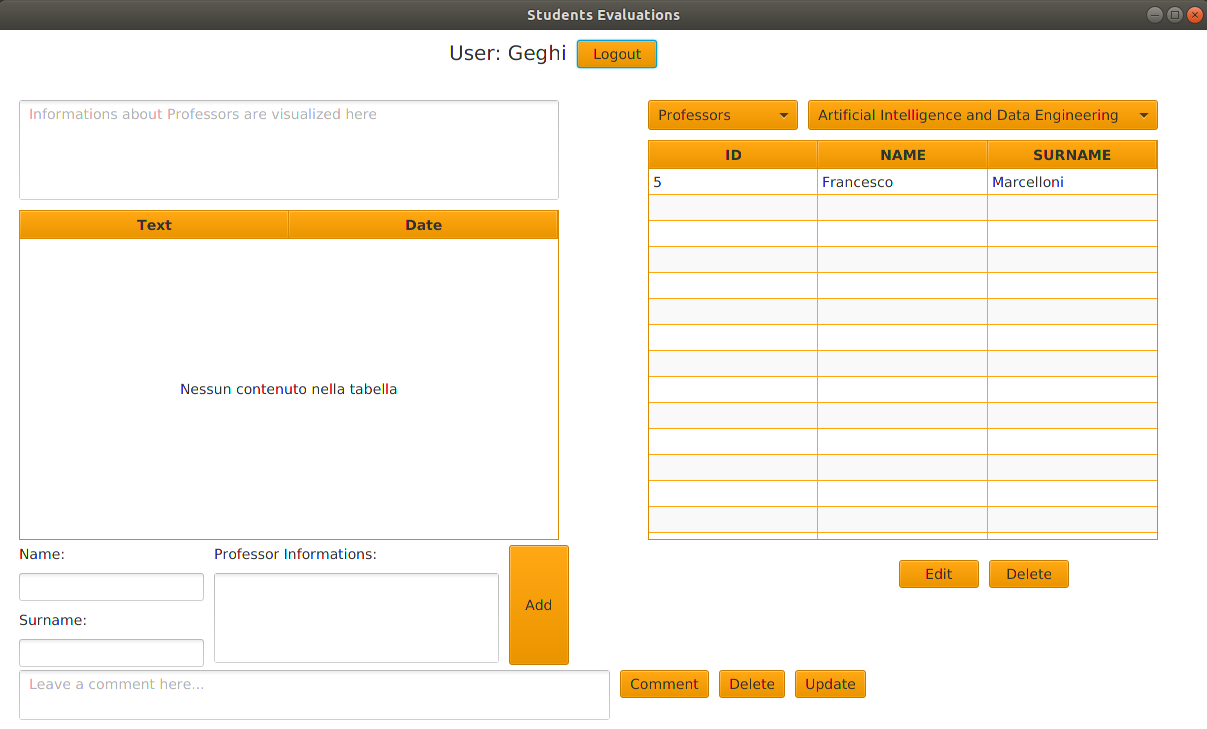
\includegraphics[width=0.88\textwidth]{images/screens/adminLogin}
\captionof{figure}{Interface after the administrator has logged in}
\label{fig:adminLogin}
\end{figure}

You can choose to add a new professor, using the input fields at the bottom left. You have to specify the name, surname, and description, then press the "Add" button (fig.~\ref{fig:admin1}).
\begin{figure}[h]
\centering
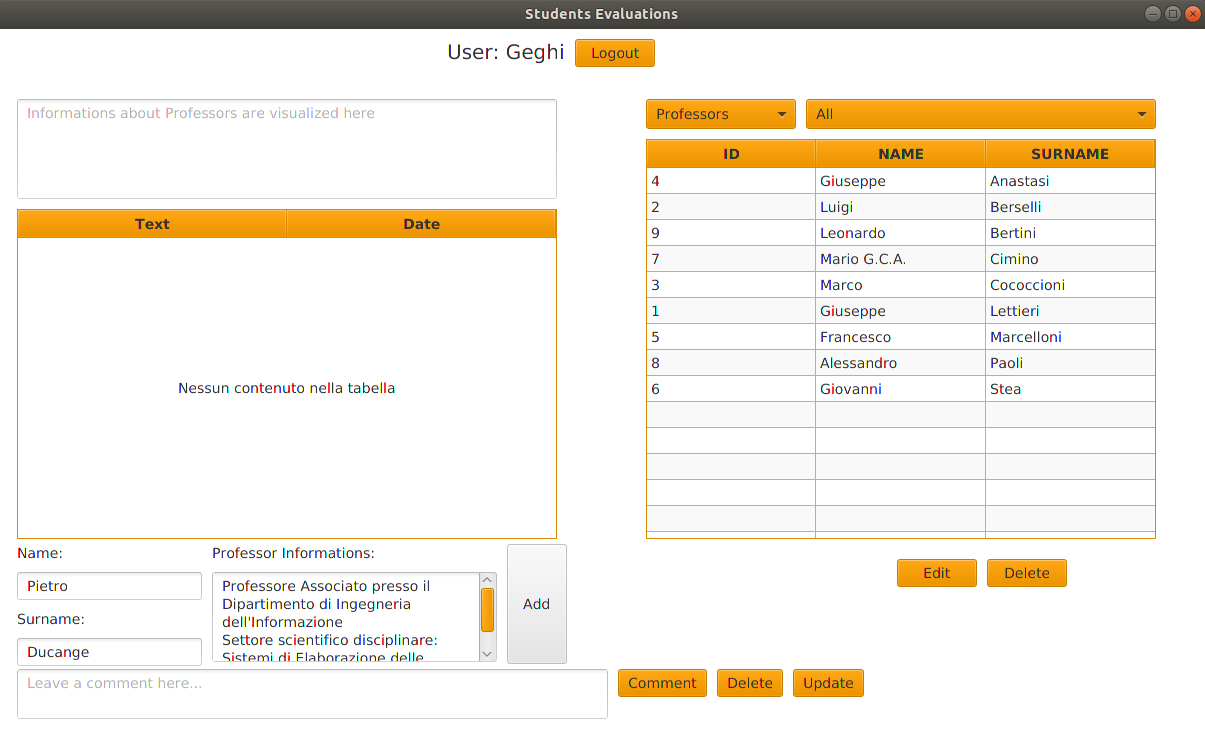
\includegraphics[width=0.88\textwidth]{images/screens/admin1}
\captionof{figure}{Adding a new professor}
\label{fig:admin1}
\end{figure}
\clearpage
You can also modify the data related to a professor: click on the professor you are interested in and change the information shown in the apposite input fields. Finally, you have the chance to delete a professor by clicking on the "Delete" button after selecting the wanted professor (fig.~\ref{fig:admin2}).
\begin{figure}[h]
\centering
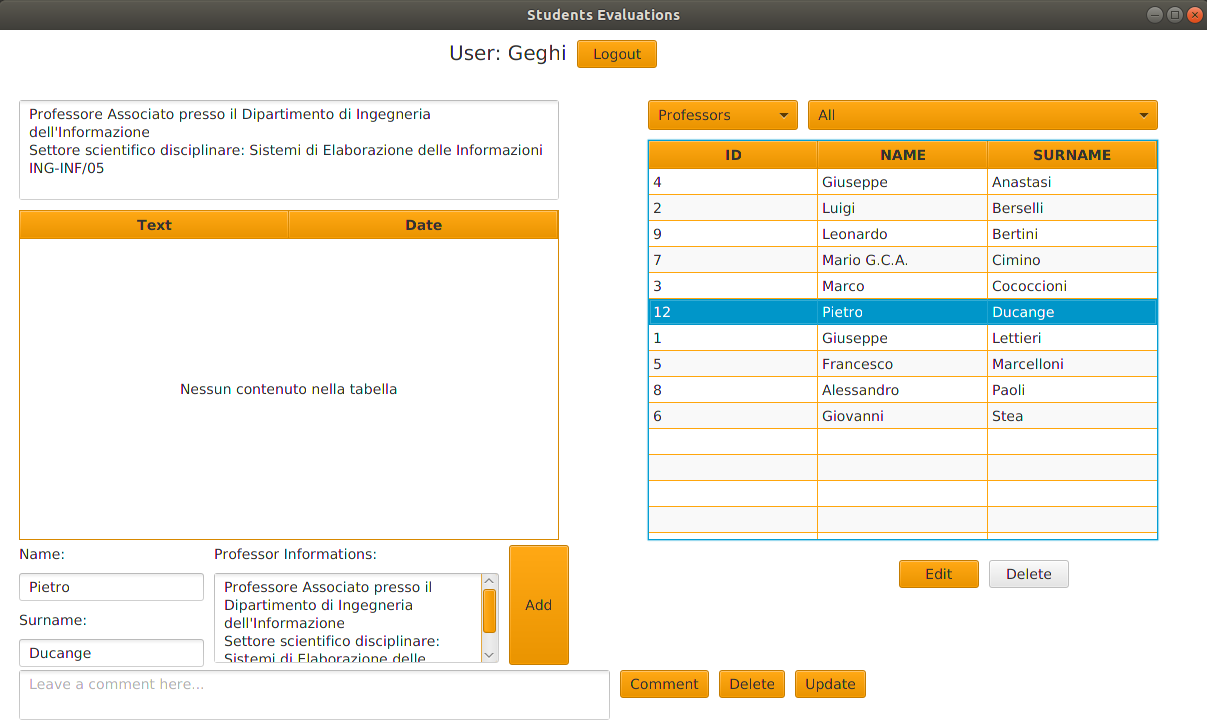
\includegraphics[width=0.88\textwidth]{images/screens/admin2}
\captionof{figure}{Screen of the application's interface from which you can either update or delete a professor}
\label{fig:admin2}
\end{figure}

All these operations are available for the subjects as well. The only difference is that when you want to add a new subject you also need to specify the id of the professor teaching it (or a list of ids, separeted by commas, if there are more professors teaching it). Moreover, you must have precisely displayed in the table the subjects of the same degree course of the new one (fig.~\ref{fig:admin3}).
\begin{figure}[h]
\centering
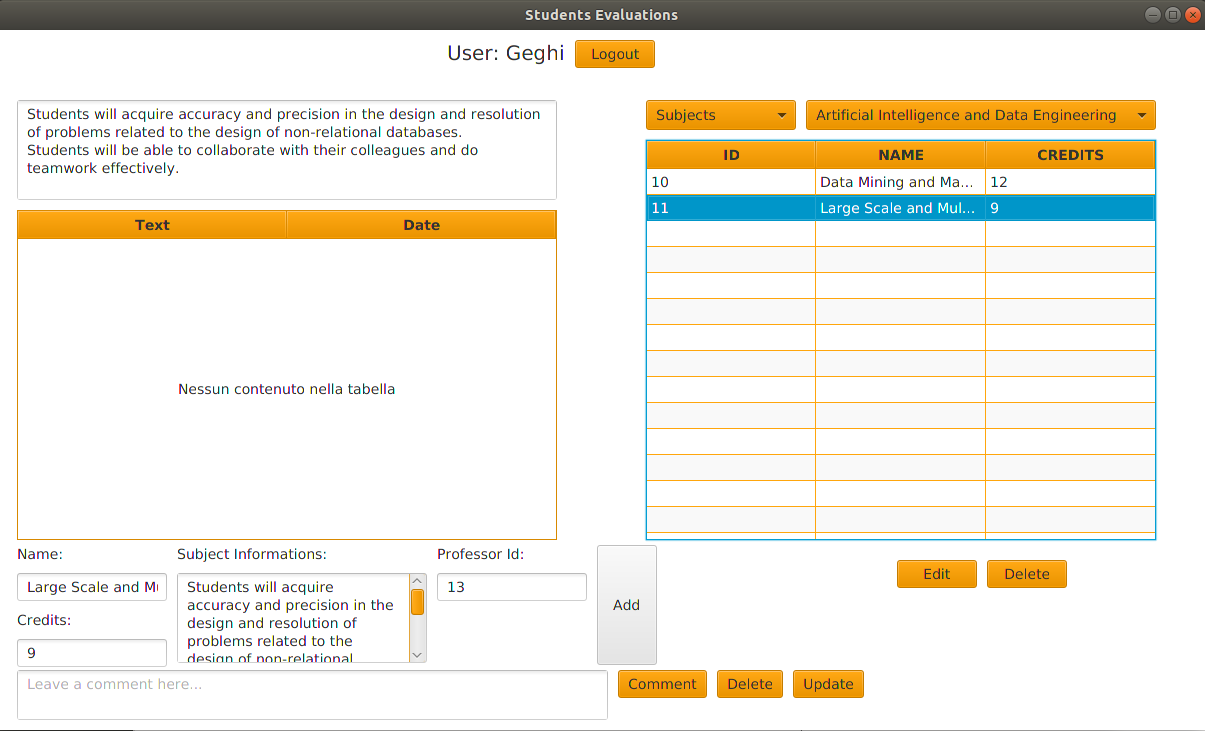
\includegraphics[width=0.88\textwidth]{images/screens/admin3}
\captionof{figure}{Interface after adding a new subject, ready to modify or delete it}
\label{fig:admin3}
\end{figure}
\clearpage
The administrator can delete comments posted by all the users, too. Just click on the comment and then on the "Delete" button (fig.~\ref{fig:admin4}).
\begin{figure}[h]
\centering
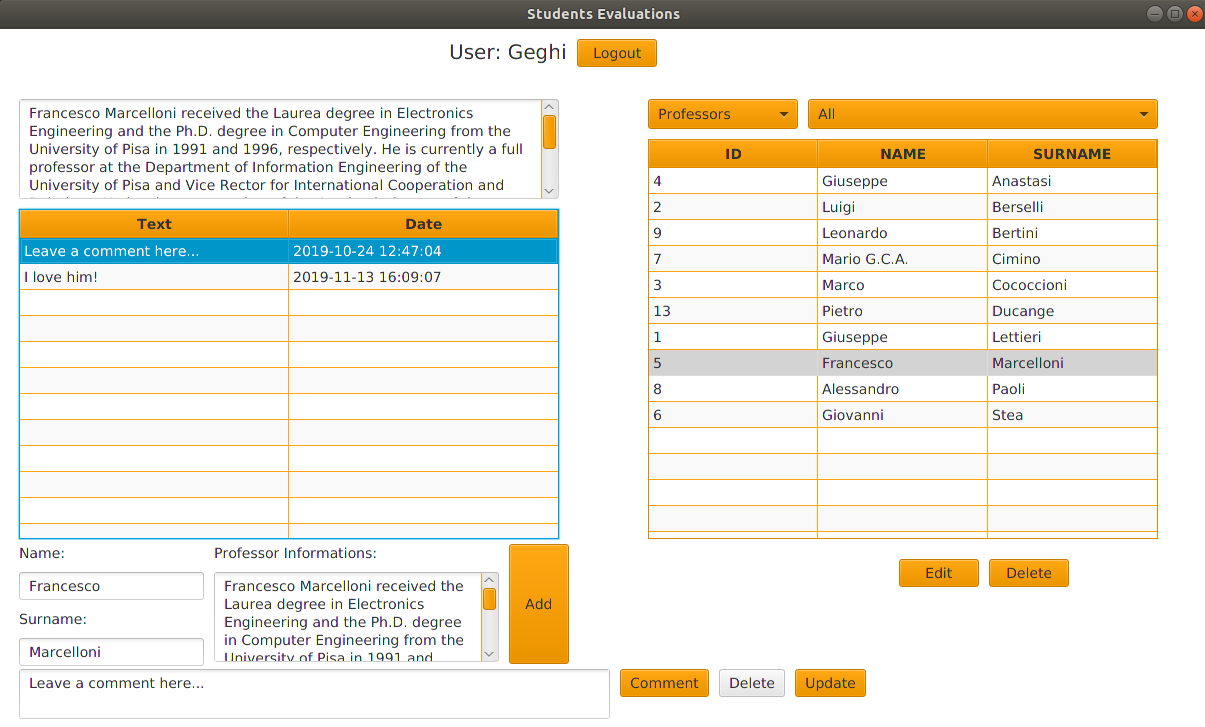
\includegraphics[width=0.88\textwidth]{images/screens/admin4}
\captionof{figure}{Screen of the application's interface from which the admin can delete a comment}
\label{fig:admin4}
\end{figure}


\end{document}






